%==============================================================================
% Sjabloon poster bachproef
%==============================================================================
% Gebaseerd op document class `a0poster' door Gerlinde Kettl en Matthias Weiser
% Aangepast voor gebruik aan HOGENT door Jens Buysse en Bert Van Vreckem

\documentclass[a0,portrait]{hogent-poster}

% Info over de opleiding
\course{Bachelorproef}
\studyprogramme{toegepaste informatica}
\academicyear{2022-2023}
\institution{Hogeschool Gent, Valentin Vaerwyckweg 1, 9000 Gent}

% Info over de bachelorproef
\title{Vergelijkende studie van Augmented Reality ondersteunde mobiliteitstool voor personen met een mentale beperking: een proof of concept.}
\subtitle{}
\author{Robin De Waegeneer}
\email{robin.dewaegeneer@student.hogent.be}
\supervisor{Sebastiaan Labijn}
\cosupervisor{Thomas Aelbrecht (Hogent)}

% Indien ingevuld, wordt deze informatie toegevoegd aan het einde van de
% abstract. Zet in commentaar als je dit niet wilt.
\specialisation{AI \& Data engineer}
\keywords{Augmented Reality, Applicatie, Navigatie}
\projectrepo{https://github.com/RobinDeWaegeneer/Bachelorproef2023RobinDeWaegeneer}

\begin{document}

\maketitle

\begin{abstract}

\end{abstract}

\begin{multicols}{2} % This is how many columns your poster will be broken into, a portrait poster is generally split into 2 columns

\section{Introductie}

\section{Experimenten}


\section{Sectie met figuur}

\begin{center}
  \captionsetup{type=figure}
  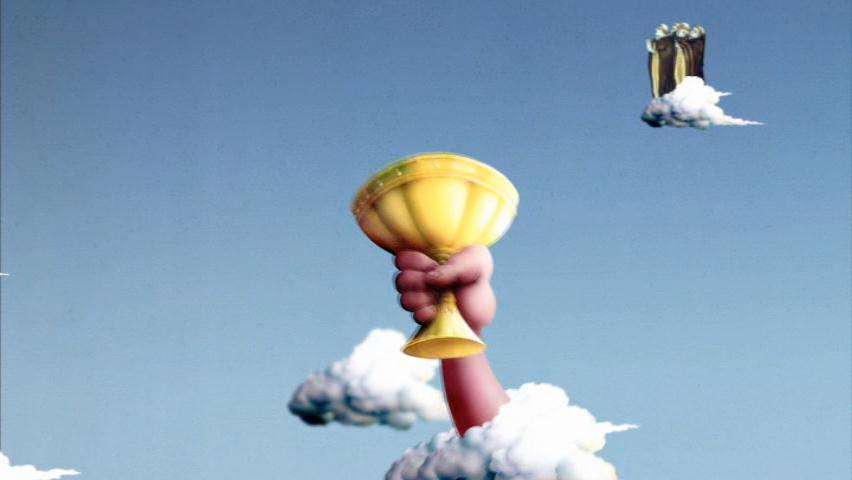
\includegraphics[width=1.0\linewidth]{grail}
  \captionof{figure}{}
\end{center}

Let er wel op dat dit tot problemen met bladschikking kan leiden.

\section{Conclusies}

\section{Toekomstig onderzoek}



\end{multicols}
\end{document}